En este capítulo procederemos a detallar la planificación que ha seguido el
proyecto. En particular, se describe la metodología seguida, las etapas por las
que ha pasado el proyecto, la planificación temporal y la organización del
personal involucrado. 

Tras ello se exponen los recursos inventariables de los
que se han hecho uso a lo largo del desarrollo y puesta en producción del
producto, haciendo una estimación de los costes y, por último, explicando los
posibles riesgos que pueden tener lugar.

En general, el desarrollo del proyecto se ha ajustado razonablemente bien al calendario
inicialmente dispuesto en la planificación, con algunas etapas durando más de lo
previsto pero otras terminando antes de lo planificado. 

\section{Metodología de desarrollo}

Para la realización del proyecto se ha utilizado un modelo de desarrollo
iterativo incremental, definiendo en cada etapa las funcionalidades a
elaborar y completando el ciclo completo de desarrollo y pruebas. 

A continuación se detallan cada una de las iteraciones por las que ha ido
pasando el proyecto.

\subsection{Primera iteración: adquisición de conocimientos y elicitación de requisitos}

Antes de poder comenzar con el análisis y diseño del propio proyecto,
era esencial adquirir una serie de conocimientos para poder afrontar
su desarrollo con todas las garantías. Durante esta iteración, se
llevaron a cabo labores de documentación y aprendizaje autodidacta con
las que se asentaron los conocimientos necesarios.

Además, durante este periodo también se definieron los requisitos que se
impondrían al sistema, y se barajaron las diferentes posibilidades de
implementación del proyecto, así como las posibles herramientas y bibliotecas de
terceros que pudieran ser de ayuda, tal y como queda reflejado en el capítulo~\ref{chap:requisitos}.

En particular, en esta etapa se decidió el uso del framework web
\textbf{Django}, las tecnologías de desarrollo \textit{front-end}\footnote{El
  desarrollo web \textit{front-end} hace referencia a la parte de una web con la
  que el usuario interactúa directamente en el navegador.} (entre otras, Sass,
Compass, jQuery y D3), el motor de tareas asíncronas para lanzar los chequeos
(Celery y RabbitMQ) y el stack de soporte del servidor (nginx, supervisord y
gunicorn).

\subsection{Segunda iteración: desarrollo de módulo de herramientas básicas de
  chequeo}

Una vez adquiridos los conocimientos necesarios, y decididas las técnicas y
herramientas para llevar aquellos a la práctica, fue obvia la necesidad de
empezar por diseñar una serie de herramientas que fuesen capaces de lanzar
chequeos contra servicios web de forma simple y aislada.

Así, se desarrolló un módulo en Python capaz de lanzar los cuatro tipos de
chequeos con los que posteriormente contaría el proyecto:
\begin{itemize}
\item Chequeo mediante paquetes \ac{ICMP} (ping) con verificación de tiempo de espera máximo.
\item Chequeo de coherencia de registros \ac{DNS}.
\item Chequeo del estado de puertos remotos.
\item Chequeo de peticiones \ac{HTTP}, tanto en su cabecera como en contenido.
\end{itemize}

Este módulo sería el motor de los chequeos que posteriormente se darían de alta
en el proyecto.

\subsection{Tercera iteración: inicio de proyecto Django y CRUD básico}

Con el módulo de chequeo desarrollado, \textit{sólo} restaba desarrollar el
resto de la aplicación alrededor de sus funcionalidades. En esta tercera
iteración se creó la estructura básica del proyecto y se inició el desarrollo de
la funcionalidad \ac{CRUD} básica.

También en esta etapa se definió el diseño visual de la aplicación: logotipo,
esquema de colores y tipografías.

\subsection{Cuarta iteración: integración del motor de tareas asíncronas}

Con la aplicación teniendo la funcionalidad básica para la creación y edición de
chequeos, el siguiente paso fue integrar un motor de tareas asíncronas que se
dedicase a revisar y lanzar los chequeos dados de alta en el sistema, guardando
el resultado de cada uno de ellos en la base de datos y generando estadísticas.

\subsection{Quinta iteración: desarrollo de la aplicación Android}

Tras concluir el desarrollo de la aplicación web, en esta etapa se desarrolló
una aplicación móvil para el sistema operativo Android que recibe notificaciones
con información sobre los resultados de los chequeos dados de alta en el sistema.

\section{Planificación temporal}
\label{sec:planificacion}
Se ha diseñado un diagrama de Gantt para reflejar la distribución de las tareas
a lo largo del tiempo (figura~\ref{fig:gantt}, en la página \pageref{fig:gantt}).

\begin{figure}[htbp]
  \centering
  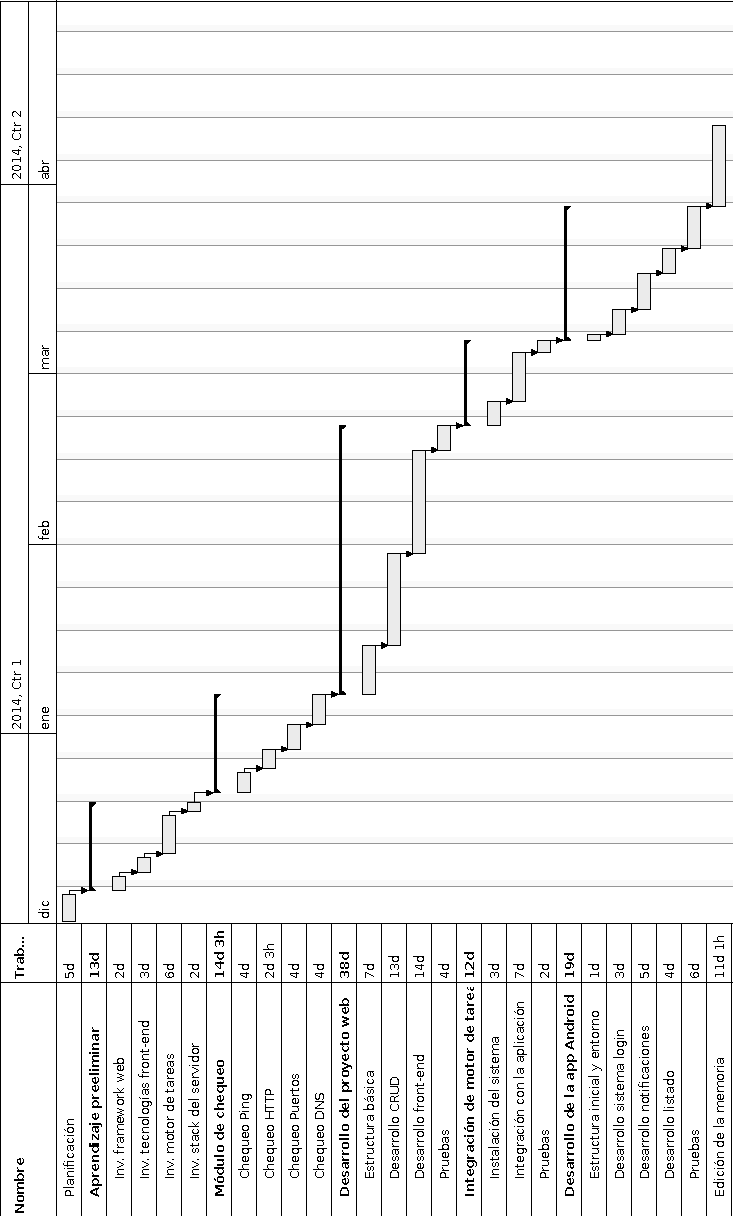
\includegraphics[width=0.9\textwidth]{2_calendario/imagen_diagrama_gantt}
  \caption{Diagrama de Gantt}
  \label{fig:gantt}
\end{figure}

Además, se presenta a continuación una comparación por fases de los plazos
estimados frente a los plazos reales tras la conclusión del proyecto.

\begin{table}[hbtp]
  \centering
  \begin{tabular}{|l|c|c|}
    \hline
    \textbf{Fase} & \textbf{Plazo estimado} & \textbf{Plazo real} \\
    \hline
    Planificación & 4 días & 5 días \\
    \hline
    Aprendizaje preeliminar & 15 días & 13 días \\
    \hline
    Módulo de chequeo & 10 días & 14 días \\
    \hline
    Plataforma web & 30 dias & 38 días \\
    \hline
    Motor de tareas & 14 días & 12 días \\
    \hline 
    Aplicación Android & 21 días & 19 días \\
    \hline
    Edición de la documentación & 28 días & 18 días \\
    \hline
  \end{tabular}
  \caption{Comparación de la estimación con los tiempos reales}
  \label{tab:estimacion_tiempo}
\end{table}

\section{Organización}

El proyecto ha sido desarrollado en su totalidad por el que escribe, alumno de
la Universidad de Cádiz, llevando a cabo las labores de análisis, diseño y
desarrollo, así como de diseño visual de las interfaces y \textit{branding} del
proyecto. El desarrollo del proyecto ha sido revisado y guiado de forma continua por el
tutor Iván Ruiz Rube.

\section{Recursos inventariables}

Los recursos de hardware utilizados durante el desarrollo y la implantación del
proyecto engloban aquellos empleados por el alumno para la elaboración del
proyecto y los necesarios para la implantación y puesta en marcha del proyecto.

En particular:
\begin{itemize}
\item Como puesto de desarrollo se ha utilizado un equipo con las siguientes características:
  \begin{itemize}
  \item Procesador Intel i5 4670k
  \item Placa Gigabyte Z87X-OC
  \item Memoria Corsair Vengeance 16GB DDR3
  \item Gráfica NVidia GeForce GTX 660 Ti
  \item SSD Crucial M4 128GB
  \item Pantalla Dell u2713H 27"
  \end{itemize}

\item Como servidores para el \textit{deployment} se han contratado los
  servicios de la empresa alemana Hetzner, haciendo uso del plan \textit{vServer
    VQ7} que proporciona un servidor virtual con las siguientes características:
  \begin{itemize}
  \item Procesador Single Core
  \item RAM 512MB
  \item Disco Duro 20GB
  \item NIC 100Mbit
  \item Tráfico máximo 1TB al mes
  \end{itemize}

\item Como dispositivo para las pruebas de la aplicación móvil se ha utilizado
  un \textbf{Samsung Galaxy Nexus} con las siguientes características:

  \begin{itemize}
  \item Sistema: Android 4.3
  \item CPU: 1.2 GHz ARM Cortex-A9 de doble núcleo.
  \item GPU: 307 MHz PowerVR SGX540.
  \item Memoria: 1 GB.
  \item Almacenamiento: 16GB
  \item Pantalla: 4.65" HD Super AMOLED, 1280x720px.
  \end{itemize}

\end{itemize}

\section{Costes}

La estimación de los costes del proyecto es divisible en dos áreas. Por un lado,
en cuanto al personal:

\begin{itemize}
\item Se requiere de un desarrollador que haga el análisis, diseño e
  implementación de la plataforma web y la aplicación Android. Según convenio~\cite{boe:convenio},
  en la categoría de \textit{Programador en Internet}, el sueldo base es de 17€/hora.
\item Se precisa de un administrador del sistemas cualificado que lleve el
  mantenimiento periódico del servidor de despliegue. Según convenio, el sueldo
  base es de 14€/hora.
\end{itemize}

Dado el contexto del proyecto, es el alumno el que cubre ambos perfiles. Por
otro lado, la infraestructura necesaria consta de:

\begin{itemize}
\item El sistema en el que se ha llevado a cabo el desarrollo. Estaba comprado
  con anterioridad al proyecto, por lo que no se ha reflejado en este despliegue
  de gastos.

\item La plataforma de despliegue del sistema. Se trata de un \ac{VPS} alquilado
  mensualmente con un coste fijo de 7.90€ al mes~\cite{hetznervq7}, impuestos
  incluidos.
\end{itemize}

Así, haciendo uso de lo dispuesto en la sección~\ref{sec:planificacion},
\textit{\nameref{sec:planificacion}} y suponiendo un periodo mínimo de actividad
de 12 meses, se elabora la tabla de planificación de gastos del cuadro~\ref{tab:costes}.

\begin{table}[hbtp]
  \centering
  \begin{tabular}[h]{|l|c|c|r|}
    \hline
    \textbf{Concepto} & \textbf{Coste unitario} & \textbf{Unidades} & \textbf{Coste total} \\
    \hline
    \textit{Desarrollador} & 17€/hora & 480 horas & 8160€ \\
    \hline
    \textit{Administrador} & 14€/hora & 48 horas & 672€ \\
    \hline
    \textit{Servidor VPS} & 7.90€/mes & 12 meses & 94.80€ \\
    \hline
    \textbf{Total} & & & \textbf{8926.80€} \\
    \hline
  \end{tabular}
  \caption{Tabla de planificación de costes}
  \label{tab:costes}
\end{table}

\section{Riesgos}

\label{sec:riesgos}

Los principales riesgos presentes en SiteUp son los siguientes.

\subsection{Compromiso de la plataforma de despliegue}
\label{subsec:riesgo-compromiso-plataforma}

Dada la limitada envergadura del proyecto por ser éste un PFC y no un desarrollo
con fines comerciales, los chequeos de los servicios web se hacen de forma
centralizada desde la plataforma de despliegue. Cualquier problema que pueda
comprometer la estabilidad de esta plataforma supone un riesgo de obtener datos
falsos de los chequeos. En un entorno real, para obtener la mayor fiabilidad y
datos siempre precisos, cada chequeo se lanza desde diversos puntos, tanto
geográficos como lógicos, de forma que es más difícil que un falso positivo o
negativo causado por un error de la plataforma pueda llegar hasta el usuario.

Lógicamente la adición de nuevas \textit{sondas} de chequeo incrementaría
enormemente la complejidad logística y el presupuesto del proyecto.

\subsection{Limitación de recursos}

SiteUp hace uso de un gran número de sistemas, desde el servidor web que recibe
las peticiones hasta la cola de tareas asíncronas. La plataforma de despliegue
cuenta con unos recursos limitados que, en situaciones de gran afluencia de
peticiones, pueden no ser suficientes y dar lugar a problemas en el
sistema. 

Este riesgo puede superarse considerando contratar planes con más recursos para
la plataforma, lo que por otro lado conllevaría un incremento en los gastos.

\subsection{Rechazo de los servicios vigilados}

Por definición, los sistemas de vigilancia tienen que lanzar chequeos de forma
periódica y repetida a lo largo del tiempo. Algunos sistemas están configurados
para detectar esta clase de comprobaciones y bloquearlas, al identificarlas (a
veces erróneamente) como ataques de denegación de servicio~\cite{ddos}. 

Este riesgo es algo que tenemos que asumir y frente al que no se puede hacer
mucho, aparte de configurar la periodicidad de las comprobaciones para
disminuir la frecuencia y que no se tomen como un ataque.



%%% Local Variables: 
%%% mode: latex
%%% TeX-master: "../memoria"
%%% End: 
